%  30 Oct 2024 11:04:37
\documentclass{article}
\usepackage{geometry,booktabs,longtable,pdflscape,rotating,threeparttable,subcaption,graphicx,float,}
\usepackage{tabularx,xcolor,colortbl,}
\usepackage{hyperref}
\hypersetup{                           colorlinks=true,                   linkcolor={blue!50!black},                    filecolor={blue!50!black},                 urlcolor={blue!80!black},                     }                              \date{}
\geometry{verbose,letterpaper,lmargin=2.5cm,tmargin=2.5cm}

\begin{document}

\title{Illustrating the use of the latexlog package}
\maketitle
A descriptive analysis of the nlsw88.dta data
\section{Introduction}
This file provides examples of the use of the latexlog package.
\section{Saving Figures}
\begin{figure}[H] 
\centering 
\begin{tabular}{p{6in}}
\caption{A scatterplot of wage vs. experience using the addfig subcommand} 
\end{tabular}
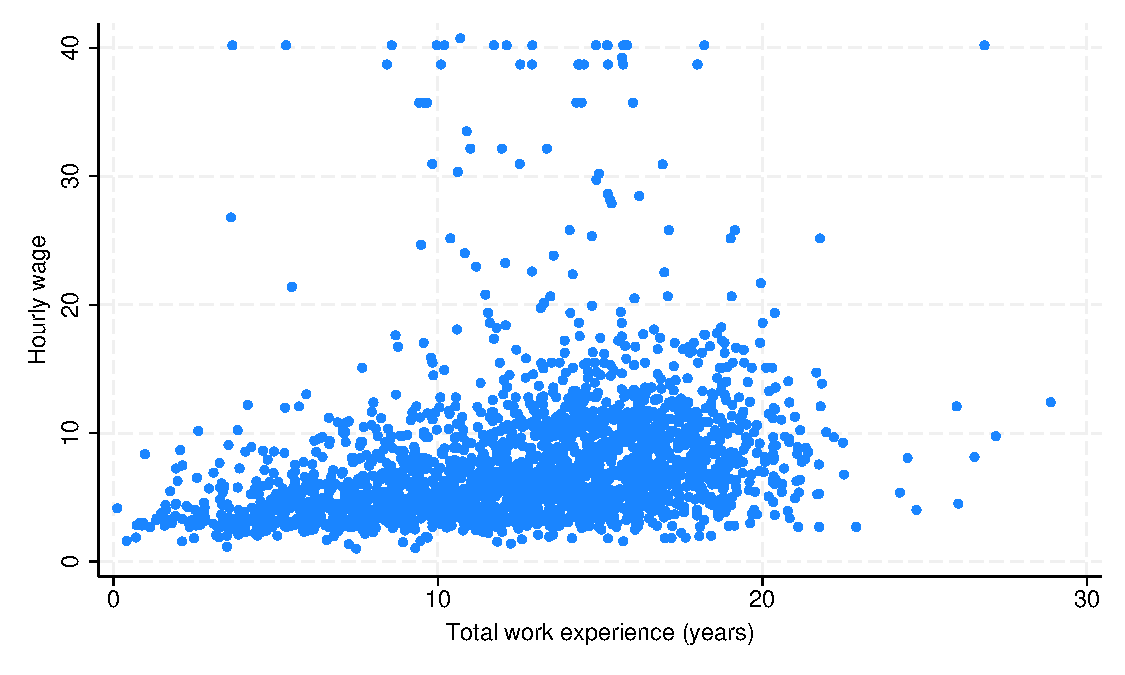
\includegraphics[width = .8\textwidth]{./figures/scatter_wage.pdf} \\ 
\begin{tabular}{p{6in}}  
\footnotesize \vspace{2pt} 
  \textbf{Notes:} Based on the nlsw88.dta data 
\end{tabular} 
\end{figure} 
\begin{figure}[H] 
\centering 
\begin{tabular}{p{6in}}
  \caption{Four Scatterplots of different variables vs. experience using the subfigure subcommand} 
\end{tabular}
\begin{subfigure}{.45\textwidth}
  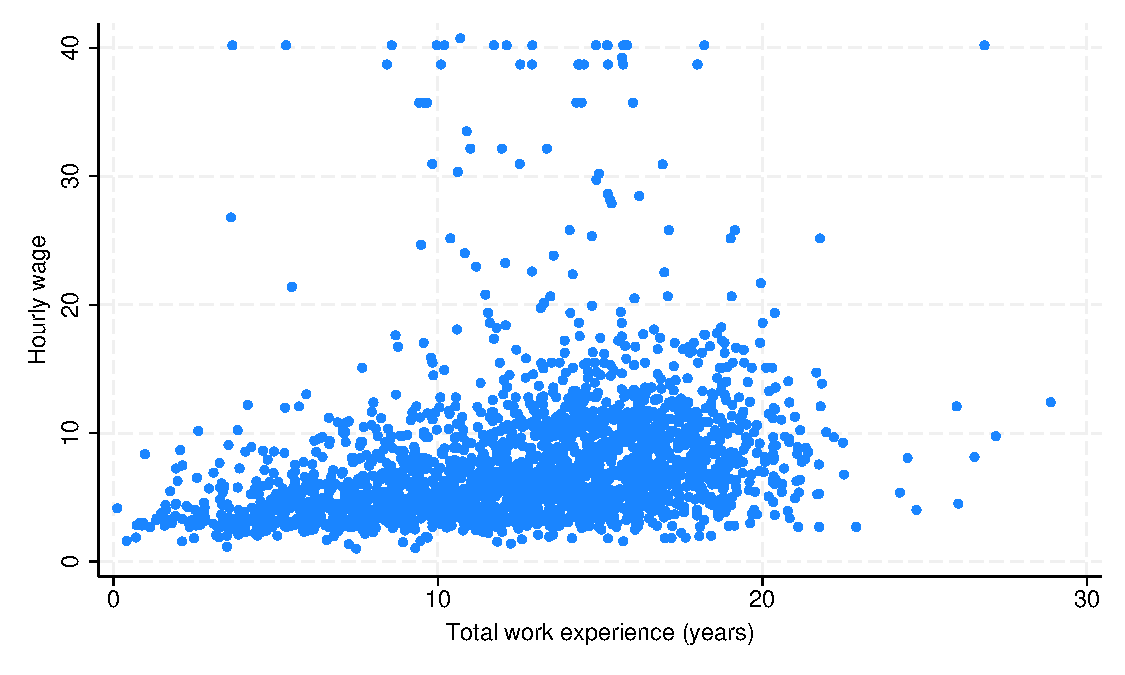
\includegraphics[width = 1.00\textwidth]{./figures/scatter_wage.pdf}  
  \caption{Hourly wage vs. experience}
\end{subfigure}
\begin{subfigure}{.45\textwidth}
  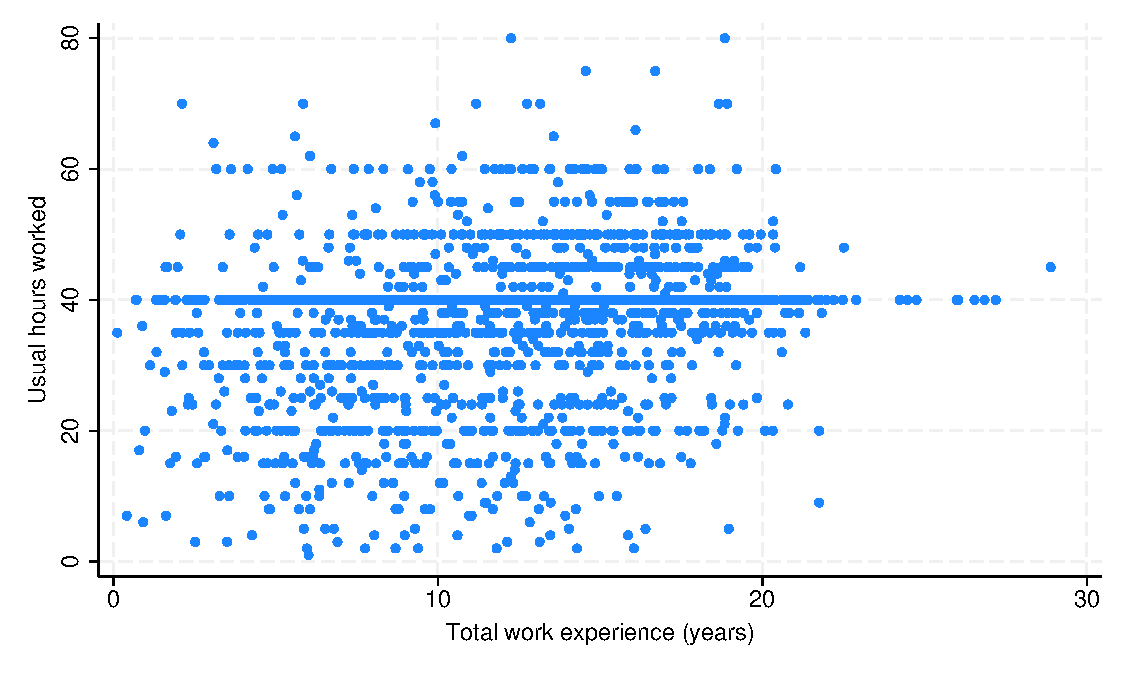
\includegraphics[width = 1.00\textwidth]{./figures/scatter_hours.pdf}  
  \caption{Usual hours worked vs. experience}
\end{subfigure}
\begin{subfigure}{.45\textwidth}
  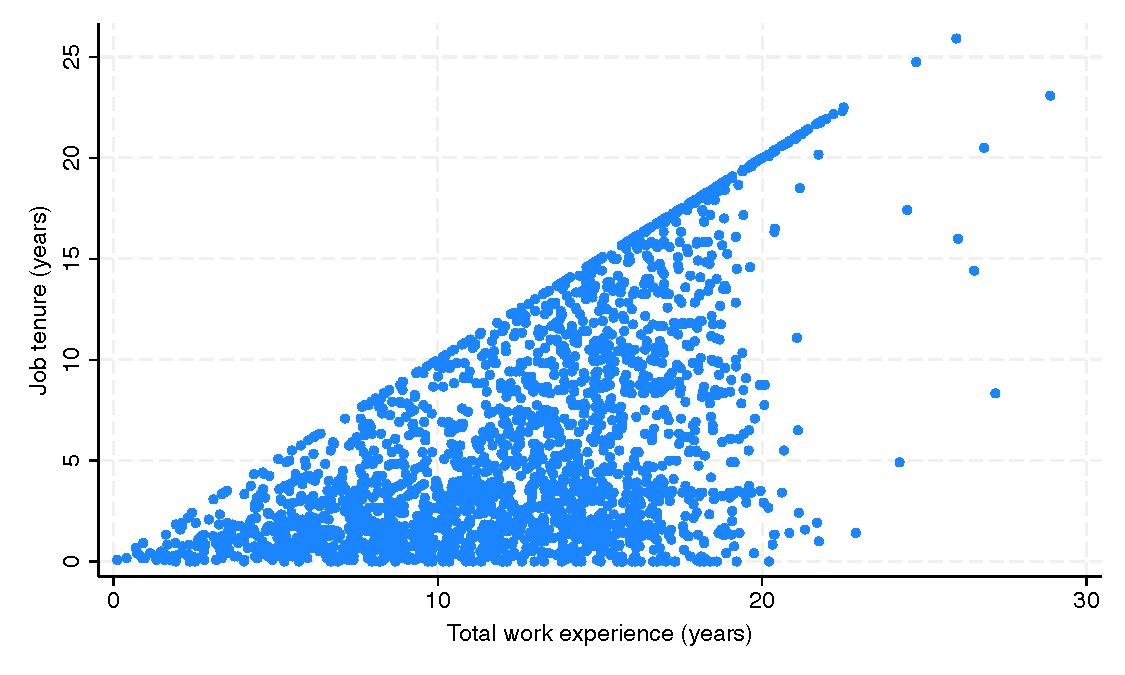
\includegraphics[width = 1.00\textwidth]{./figures/scatter_tenure.pdf}  
  \caption{Job tenure (years) vs. experience}
\end{subfigure}
\begin{subfigure}{.45\textwidth}
  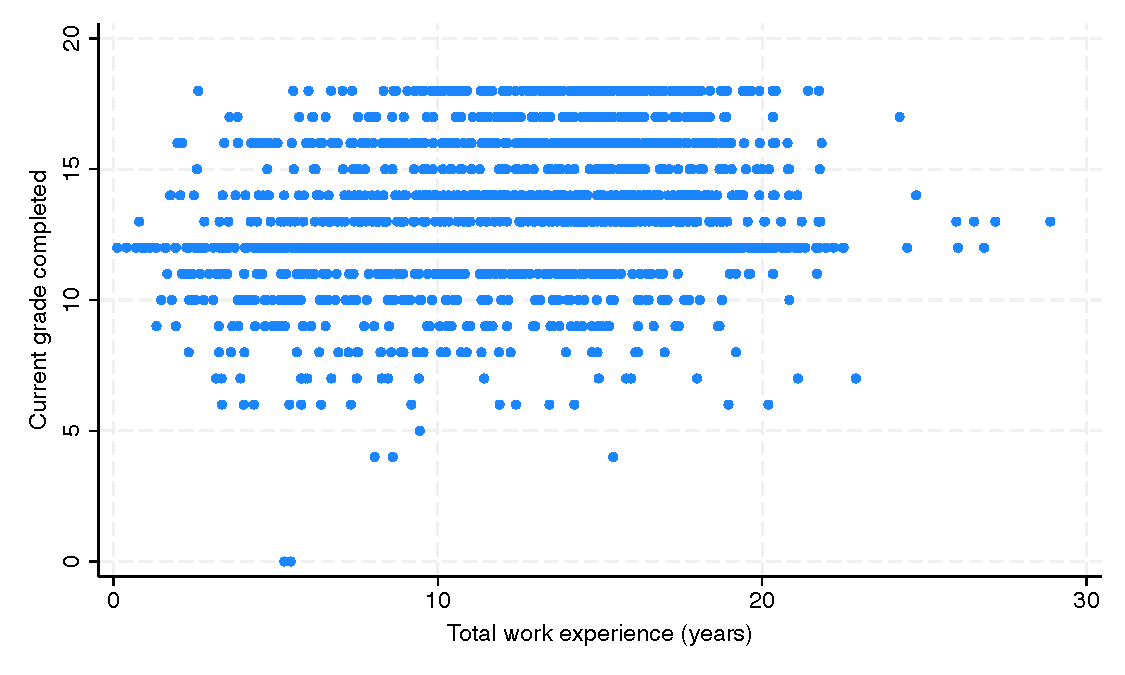
\includegraphics[width = 1.00\textwidth]{./figures/scatter_grade.pdf}  
  \caption{Current grade completed vs. experience}
\end{subfigure}
\begin{tabular}{p{6in}}  
 \footnotesize \vspace{2pt} 
 \textbf{Notes:} Based on the nlsw88.dta data 
\end{tabular} 
\end{figure} 
\clearpage\pagebreak
\section{Saving Tables with latexlog}
\subsection{Example of a twoway table:}
The following example creates a twoway table using Stata's \textbf{table} command. 
This table is then saved to the log file using the \textbf{collect export} subcommand.
\begin{table}[htbp] 
\centering 
\begin{threeparttable} 
\caption{Table using Stata table command and latexlog collect export subcommand} 

\centering
\begin{tabular}{lll}
\toprule
\multicolumn{1}{c}{} &
  \multicolumn{2}{c}{Union worker} \\
\multicolumn{1}{c}{} &
  \multicolumn{1}{r}{Nonunion} &
  \multicolumn{1}{r}{Union} \\
\midrule
\multicolumn{1}{l}{Occupation} &
  \multicolumn{1}{r}{} &
  \multicolumn{1}{r}{} \\
\multicolumn{1}{l}{\hspace{1em}Professional/Technical} &
  \multicolumn{1}{r}{208} &
  \multicolumn{1}{r}{66} \\
\multicolumn{1}{l}{\hspace{1em}Managers/Admin} &
  \multicolumn{1}{r}{204} &
  \multicolumn{1}{r}{19} \\
\multicolumn{1}{l}{\hspace{1em}Sales} &
  \multicolumn{1}{r}{468} &
  \multicolumn{1}{r}{145} \\
\multicolumn{1}{l}{\hspace{1em}Clerical/Unskilled} &
  \multicolumn{1}{r}{70} &
  \multicolumn{1}{r}{5} \\
\multicolumn{1}{l}{\hspace{1em}Craftsmen} &
  \multicolumn{1}{r}{40} &
  \multicolumn{1}{r}{10} \\
\multicolumn{1}{l}{\hspace{1em}Operatives} &
  \multicolumn{1}{r}{128} &
  \multicolumn{1}{r}{83} \\
\multicolumn{1}{l}{\hspace{1em}Transport} &
  \multicolumn{1}{r}{19} &
  \multicolumn{1}{r}{1} \\
\multicolumn{1}{l}{\hspace{1em}Laborers} &
  \multicolumn{1}{r}{171} &
  \multicolumn{1}{r}{35} \\
\multicolumn{1}{l}{\hspace{1em}Farmers} &
  \multicolumn{1}{r}{1} &
  \multicolumn{1}{r}{} \\
\multicolumn{1}{l}{\hspace{1em}Farm laborers} &
  \multicolumn{1}{r}{6} &
  \multicolumn{1}{r}{1} \\
\multicolumn{1}{l}{\hspace{1em}Service} &
  \multicolumn{1}{r}{7} &
  \multicolumn{1}{r}{5} \\
\multicolumn{1}{l}{\hspace{1em}Household workers} &
  \multicolumn{1}{r}{} &
  \multicolumn{1}{r}{1} \\
\multicolumn{1}{l}{\hspace{1em}Other} &
  \multicolumn{1}{r}{87} &
  \multicolumn{1}{r}{89} \\
\bottomrule
\end{tabular}

 \footnotesize  
\textbf{Notes:} Command: table occupation union, nototals 
\end{threeparttable} 
\end{table}
\subsection{Example of a regression table:}
\begin{table}[htbp] 
\centering 
\begin{threeparttable} 
\caption{Regression Table using Stata etable command and latexlog collect export subcommand} 

\centering
\begin{tabular}{lll}
\toprule
\multicolumn{1}{r}{} &
  \multicolumn{1}{c}{logwage} &
  \multicolumn{1}{c}{logwage} \\
\midrule
\multicolumn{1}{l}{Total work experience (years)} &
  \multicolumn{1}{r}{0.048} &
  \multicolumn{1}{r}{0.039} \\
\multicolumn{1}{l}{} &
  \multicolumn{1}{r}{(0.002)} &
  \multicolumn{1}{r}{(0.002)} \\
\multicolumn{1}{l}{Current grade completed} &
  \multicolumn{1}{r}{} &
  \multicolumn{1}{r}{0.081} \\
\multicolumn{1}{l}{} &
  \multicolumn{1}{r}{} &
  \multicolumn{1}{r}{(0.004)} \\
\multicolumn{1}{l}{Married} &
  \multicolumn{1}{r}{} &
  \multicolumn{1}{r}{-0.007} \\
\multicolumn{1}{l}{} &
  \multicolumn{1}{r}{} &
  \multicolumn{1}{r}{(0.022)} \\
\multicolumn{1}{l}{Intercept} &
  \multicolumn{1}{r}{1.267} &
  \multicolumn{1}{r}{0.325} \\
\multicolumn{1}{l}{} &
  \multicolumn{1}{r}{(0.032)} &
  \multicolumn{1}{r}{(0.060)} \\
\multicolumn{1}{l}{Number of observations} &
  \multicolumn{1}{r}{2246} &
  \multicolumn{1}{r}{2244} \\
\multicolumn{1}{l}{Adjusted R-squared} &
  \multicolumn{1}{r}{0.15} &
  \multicolumn{1}{r}{0.27} \\
\bottomrule
\end{tabular}

 \footnotesize  
\textbf{Notes:} Command: etable, estimates(model1 model2) mstat(N) mstat(r2\_a) 
\end{threeparttable} 
\end{table}

\end{document}
